\documentclass[10pt,letterpaper]{article}

\usepackage{cogsci}
\usepackage{pslatex}
\usepackage{apacite}
\usepackage{amsmath}
\usepackage{float} 
\usepackage{graphicx}

%Comment out for submission
\cogscifinalcopy

\title{Rapid Presentation Rates Negatively Impacts the Contiguity Effect In Free Recall}
 
\author{{\large \bf Claudio Toro-Serey (ctoro@bu.edu), Ian M. Bright (imbright@bu.edu), and Marc W. Howard (marc777@bu.edu)} \\
  Department of Psychological and Brain Sciences, 64 Cummington Mall\\
  Boston, MA 02215 USA}


\begin{document}

\maketitle


\begin{abstract}
A prevalent finding in memory research is that recalling a previously studied item incurs a jump back in time, such that items temporally contiguous to the recalled element have a higher probability of being subsequently remembered. While widely explored, a remaining open question concerning this contiguity effect is the extent to which the presentation rate of study lists impacts this form of temporal binding. Here, we explore the persistence of the contiguity effect at presentation rates from 2Hz to 8Hz. Our results show that temporal binding was negatively correlated with rate, and significantly diminished for a presentation rate of 8hz. This frequency matches the upper bound of neural-related theta frequency, which has been linked to temporal encoding of episodic memories. However, we also found a diminished effect of semantic relatedness, thus raising the question of whether presentation rate is directly affecting encoding, subsequent recall, or both.

\textbf{Keywords:} 
Words, words, words, words
\end{abstract}

\section{Introduction}

Cognitive neuroscientists have hypothesized that the successful retrieval of an episodic memory is accompanied by a ``jump back in time,'' a recovery of the previous memory's context. \cite{Tulv83}
In free recall studies, this recovery manifests as the contiguity effect, wherein after the successful recall of an item, the next item to be recalled is more likely to be a close temporal neighbor than a more distant one \cite{Kaha96}. 
This distance is measured as lag, a directed distance between any two items in a study list. For example, in the list ``absence, hollow, pupil, river, darling'', the lag from absence to river is 3, while the lag from darling to pupil is -2. 
This effect is robust, appearing across a variety of methodological manipulations \cite{Kaha12}. 
A persistent component of the contiguity effect is its asymmetry, such that forward transitions are more likely to take place than backward transitions of the same distance. 
This asymmetry appears in all free recall studies that have looked at output order effects \cite{KahaEtal08}. 
The contiguity effect persists at presentation rates up to at least 2 Hz., but it is unknown if it persists at higher presentation rates \cite{Kaha96}. 
It is possible that increasing the presentation rate of items could interfere with whatever mechanisms in the brain allow for the temporal binding of presented items. 

Beyond the contiguity effect, free recall contains many other well-explored patterns of behavior. Consistent with a slowly changing temporal context, individuals exhibit a strong recency effect during a standard free recall task \cite{SedeEtal08}. 
That is, they are more likely to recall items presented during the end of the study period. Another robust finding is that participants are more likely to recall items from the beginning of a studied list \cite{Murd62}. 
The relative strength of these two effects is not constant, however. Davelaar et al. (2005), found that fast presentation rates during the study period (i.e., 10 Hz.) resulted in a primacy effect that was stronger than the recency effect. 
This ratio was in contrast to slower presentation rates (i.e., 5, 2.5, and 1.25 Hz.) where the recency effect was stronger than the primacy effect. 
Recency and primacy effects also manifest at the very beginning of recall. Individuals are more likely to begin recall at the beginning or end of a list, with a higher probability for more recent items \cite{HowaKaha99}. The effect of high presentation rates on the probability of first recall has yet to be reported. 

\nocite{DaveEtal05}

Across these effects, there exist outstanding questions as to the impact of fast presentation rates. Therefore, in this study we investigated the impacts of presentation rate on free recall, focusing mainly on its modulation of lag-related contiguity response probabilities (CRP). Two hypotheses drive this study. First, we hypothesized that as presentation rates increase, the temporal order of items fails to be encoded. In this event, one would expect to find a flattening of the contiguity effect. Second, concerning recency and primacy effects, we expected that there would be a shift in the ratio between primacy and recency as presentation rate increases. While Davelaar et al. (2005) demonstrated a flip in the ratio between the primacy and recency effects for overall recall between 10 Hz and slower presentation rates, they did not report the probability of first recall (PFR). Thus, we examine this measure, expecting to also find a shift in the PFR ratio as rate increases. 

\nocite{DaveEtal05}

\section{Methods}

\subsection{Subjects}

Three hundred thirty undergraduates from Syracuse University participated in this study.  
%Need more Demographic Information,
Participants were excluded if they failed to recall a correct word in at least one trial ($n = 15$), and if they did not perform all three conditions ($n = 7$). The final number of participants was 308.

\subsection{Procedure}

%Where are the words from? Toronto Word Pool? Only nouns?
Here are a few sentences about the words used and if any words were excluded. Participants took part in 18 trials. Words were presented at three presentations rates: 2 Hz., 4 Hz., and 8 Hz. 
Participants completed six trials in each condition. The order of the trials was random to control for any sequential effect.
Following the study period in each trial, participants were prompted to verbally recall as many words as possible from the list. 
Participant responses were recorded and later parsed using a semi-automatic speech parsing algorithm.

\subsection{Analysis}

We measured whether presentation rate affected either the average number of valid recalls in a trial or median response latencies. To do this, we performed a repeated measures ANOVA on each metric, with condition as the repeated factor per participant. Post-hoc paired permutations (5000 iterations) and Cohen's D effect sizes on mean recalls and median response latencies were then performed to determine significant differences. Serial position curves (SPC), were computed to show the overall probability of a word being recalled based on its position in the list for each subject. We examined whether the recency effect changed in relation to the primacy effect as a function of presentation rate. We performed a mixed effects linear regression with subject as a mixed effect and condition as fixed effect, in order to predict the difference in the probability of recall for the first and last items in the list (i.e. probability for position 20 minus probability for position 1). 

To measure the PFR, we extracted the position of the first item recalled per study list, and divided the number of times each position was recalled first over the total number of first recalls per participant. We then averaged these probabilities across participants per condition. Finally, we calculated the conditional response probability (CRP) for each lag by dividing the number of correct recall transitions at a given lag by the total number of possible correct transitions at that lag. In order to test for differences in the CRP at each lag across conditions, we performed a mixed-effects logistic regression, estimating the probability of recall for an item as a function of the interaction between the following fixed-effects predictors: absolute lag, its direction (backwards or forwards from the previously recalled item), and the presentation rate. We report Z- and T-scored coefficients for all mixed-effects models.

\section{Results}

\subsection{Overall Performance Decreases, But Becomes Faster as Presentation Rate Increases}
%Alternate subsection title: As Presentation Rate Increases, fewer words are recalled but are recalled faster.

As shown in Figure~\ref{Descriptives}, the total number of words recalled decreased as presentation rates increased (2 Hz.: mean = 3.54, SD = 0.85; 4 Hz.: mean = 2.86, SD = 0.662; 8 Hz.: mean = 2.41, SD = 0.62; rmANOVA: $F(2, 614) = 309.2, p < 0.001$). Latencies also decreased as presentation rate increased (2 Hz.: median = 1196 ms, SD = 517 ms; 4 Hz.: median = 995 ms, SD = 401 ms; 8 Hz.: median = 910 ms, SD = 392 ms; rmANOVA: $F(2, 614) = 61.38, p < 0.001$). Post-hoc paired permutations confirmed these results, showing that the presentation rate of 2 Hz. yielded significantly higher number of recalls than 4 Hz. ($p < 0.001$, Cohen's D $= 0.9$) and 8 Hz. ($p < 0.001$, Cohen's D $= 1.5$), and that 4 Hz. produced significantly more recalls than 8 Hz ($p < 0.001$, Cohen's D $= 0.69$). Similarly, overall recalls in the 2 Hz. condition were significantly slower than for 4 Hz. ($p < 0.001$, Cohen's D $= 0.4$) and 8 Hz. ($p < 0.001$, Cohen's D $= 0.64$), with 8 Hz. producing the fastest responses ($p < 0.001$, Cohen's D $= 0.22$). 
%The decrease in latency as a function of presentation rate could be due to the fewer amount of items recalled, as items remembered later during the trial could have taken longer to be produced.

\begin{figure}[H]
\begin{center}
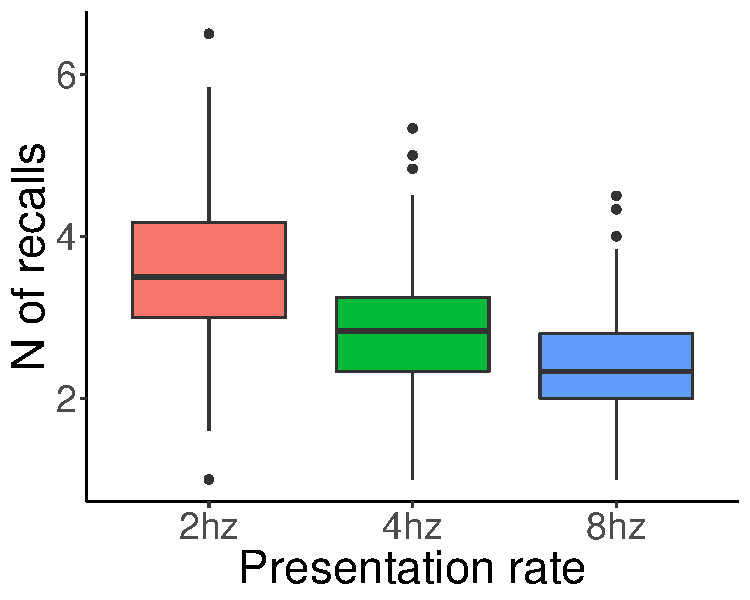
\includegraphics[width = .23\textwidth]{Images/recall_boxplot.pdf}
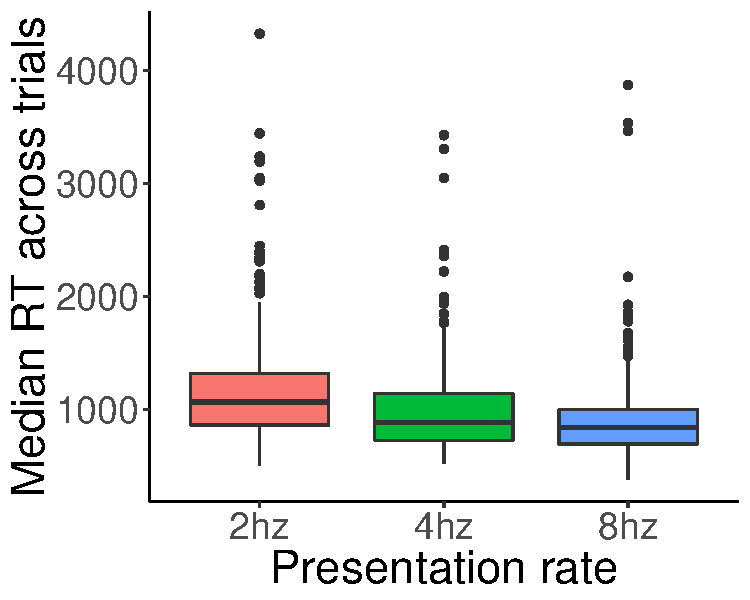
\includegraphics[width = .23\textwidth]{Images/rt_boxplot.pdf}
\end{center}
\caption{Left: Mean number of valid words recalled per trial across participants and presentation rates. The average number of recalled words decreased as presentation rate increased. Right: Median latencies (ms) across trials for each participant and presentation rate. Median latencies between valid recalls decreased as presentation rate increased} 
\label{Descriptives}
\end{figure}

\subsection{Increasing Presentation Rates Increases the Strength of the Recency Effect in Relation to the Primacy Effect}
%Too Wordy, need to change

\begin{figure}[H]
\begin{center}
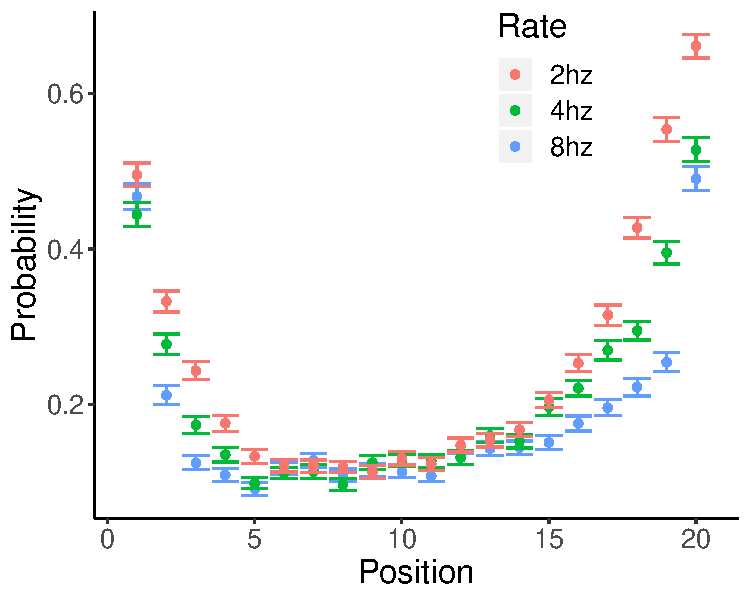
\includegraphics[width = .4\textwidth]{Images/SPC_adjusted.pdf}
\end{center}
\caption{Probability of recall as a function of position in study list. Participants showed the highest level of performance for items at the beginning and end of the list. As presentation rate increased, participants showed a tendency to have a lower recency effect in comparison to the primacy effect} 
\label{SPC}
\end{figure}

Participants showed a higher rate of recalling words from the beginning and end of a list compared to words in the middle. (Figure~\ref{SPC}). A mixed-effects linear regression showed that the probability to recall the last item on the list was higher than for the first item at 2 Hz. ($t = 6.63, p < 0.001$) and 4 Hz. ($t = 3.27, p < 0.01$), but not 8 Hz. ($t = 0.86, p = 0.38$). Comparisons among the rates showed that the recency effect was higher then the primacy effect for 2 Hz. compared to 4 Hz. ($t = -3.25, p < 0.01$) and 8hz ($t = -5.56, p < 0.001$), as well as greater for 4 Hz. compared to 8hz ($t = -2.31, p < 0.05$). %Need exact p-value
These results are in agreement with those from Davelaar et al. (2005), and show that the prominence of recency effects declines as the presentation rate increases. In terms of the PFR, participants were more likely to begin recall by reporting a word at the beginning or end of the list (Figure~\ref{PFR}). In agreement with our hypothesis, as presentation rate increased, the probability of first recall shifted from showing a stronger recency effect to a stronger primacy effect. This shift resulted in a flip such that the probability of first recall was higher for the last item on the list than the first item for a 2 Hz. presentation rate, but lower in the 8 Hz. condition.
\nocite{DaveEtal05}

\begin{figure}[H]
\begin{center}
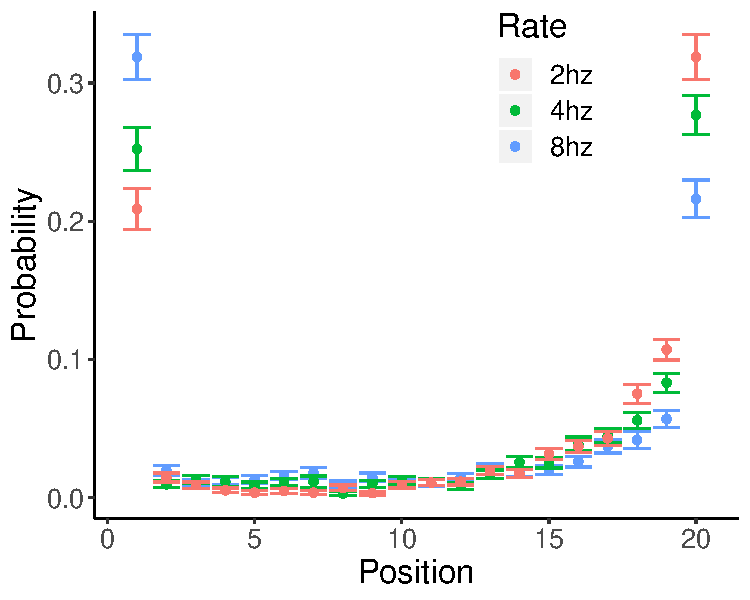
\includegraphics[width = .4\textwidth]{Images/PFR_adjusted.pdf}
\end{center}
\caption{Probability of first recall. Participants tended to begin recall by naming an item from the beginning or end of the list. At lower presentation rates, participants showed a tendency to start recall at the end of the list rather than the beginning, but this tendency flipped for high presentation rates.} 
\label{PFR}
\end{figure}

\subsection{The Contiguity Effect Flattens At Higher Presentation Rates}


Figure~\ref{uCRP} shows that after the successful recall of a word, participants were more likely to recall a word that was presented closer in time to the recalled word rather than one further away in the list. As expected, the strength of this effect decreased as presentation rate increased.
Primacy and recency can be a confound in looking at the contiguity effect. Therefore, we recalculated the CRP using only transitions that came from items from the middle of the list (serial positions 7-13). Figure~\ref{CRP} shows that there is a reduction in temporal binding as the presentation rate increases. A mixed effect logistic regression showed that forwards transitions were more probable than backwards transitions ($z = 4.18, p<0.001$), more distant transitions were less probable ($z=-4.83, p<0.001$), probabilities were higher for 2 Hz. compared to 4 Hz. ($z=-2.28, p=0.02$) and 8 Hz. ($z=-3.63, p<0.001$), the effect of absolute lag was stronger for forwards transitions than backwards transitions ($z=-2.71, p<0.01$), and the effect of lag was stronger for 2 Hz. compared to 4 Hz. ($z=2.11, p=0.03$) and 8 Hz. ($z=3.12, p<0.01$). These results confirm the trends seen in figure 5, and show that increasing the presentation rate of study words has a negative effect in the temporal binding of items in memory, particularly at 8Hz.

\begin{figure}[H]
\begin{center}
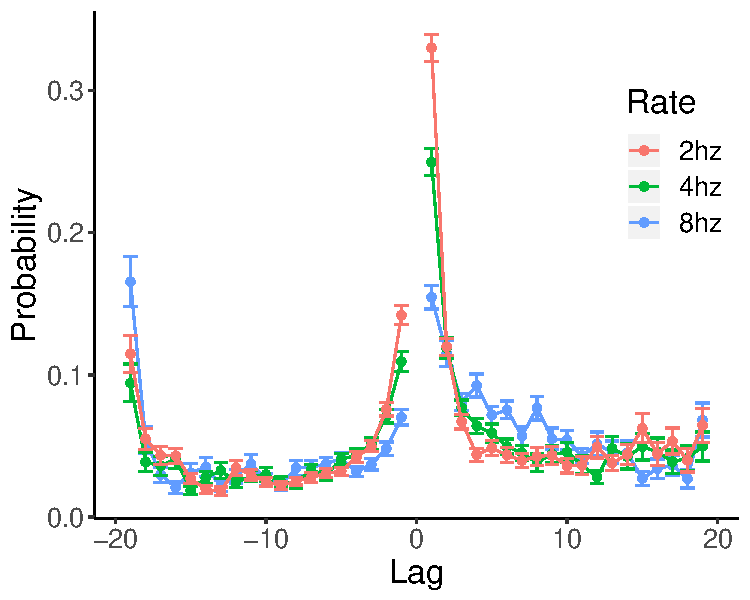
\includegraphics[width = .4\textwidth]{Images/CRP_unadjusted.pdf}
\end{center}
\caption{Lag CRP for all presentation rates. Contiguity effect visibly diminishes as presentation rate increases.} 
\label{uCRP}
\end{figure}

\begin{figure}[H]
\begin{center}
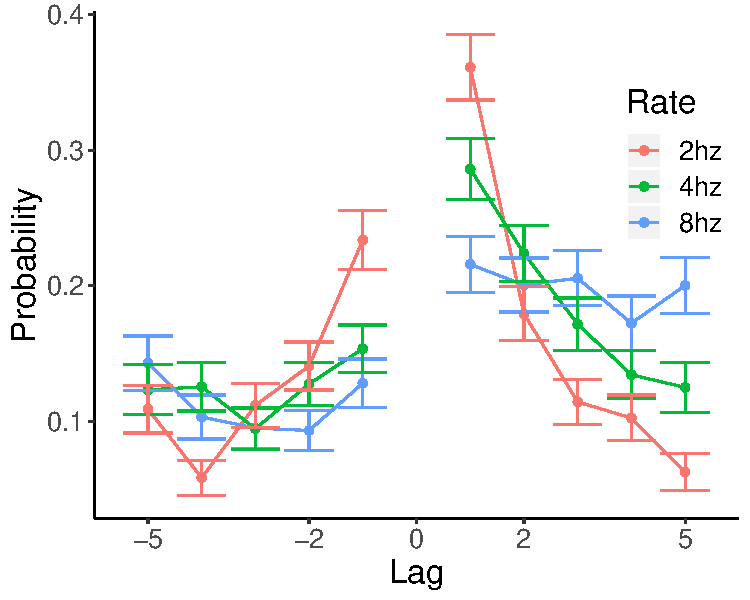
\includegraphics[width = .4\textwidth]{Images/CRP_adjusted.pdf}
\end{center}
\caption{Lag CRP adjusted for primacy and recency effects. As presentation rates increase, the contiguity effect weakens but remains asymmetric.} 
\label{CRP}
\end{figure}


\section{Discussion}

Remembering past events is associated with a jump back in time, manifesting in a higher probability for temporally contiguous elements to be subsequently recalled. In this study, we investigated whether higher presentation rates would negatively impact our ability to engender this relationship. The temporal binding of items was inhibited in the 8 Hz. condition. This inhibition manifested as a flattening of the contiguity effect. Furthermore, there was a pronounced asymmetry between forward and backward transition probabilities, consistent with a failure to build temporal associations while maintaining an ability to recover a previous state of contextual drift. In addition to these findings, our results were consistent with previous free recall studies. For instance, the average number of words recalled per list decreased as the presentation rate increased. Also, as the presentation rate increased, the strength of the primacy effect increased compared to the recency effect. A novel finding was that individuals were more likely to initiate recall with the first item on the list in the 8 Hz. condition, whereas recall of the last item was more likely in the other conditions.

 Our results pose questions about the relation of presentation rate and neural coding. Medial temporal lobe theta (3-8Hz) is related to successful encoding in free recall, particularly when binding elements temporally \cite{NyhuCurr10}. In addition, Guderian and colleagues (2009) have shown that prediction of successfully-recalled items relies on theta frequency. While presentation rates of 2hz and 4hz are mostly contained within this frequency, 8hz lies at the upper bound of theta. It is possible that our presenting 8 words per second can outpace the brain's ability to temporally associate the elements at hand, thus explaining why lag CRPs become weaker for this presentation speed. Examination of encoding and retrieval periods using EEG could help address this issue in the future. These results suggest further experiments are necessary. The contiguity effect manifests in some way in a variety of memory paradigms. If temporal binding does break down at high speeds, the contiguity effect should also diminish in these other paradigms. From a neural perspective, this paradigm falls naturally into EEG/MEG examinations. This would enable a fuller understanding of any links between theta oscillations in the brain, and temporal binding.

\nocite{GudeEtal09}


\bibliographystyle{apacite}

\setlength{\bibleftmargin}{.125in}
\setlength{\bibindent}{-\bibleftmargin}

\bibliography{bibdesk}


\end{document}